\section{Nota teórica}
\subsection*{Microcontrolador ATTiny4313}
%%%
%\begin{figure}[H]
%\centering
%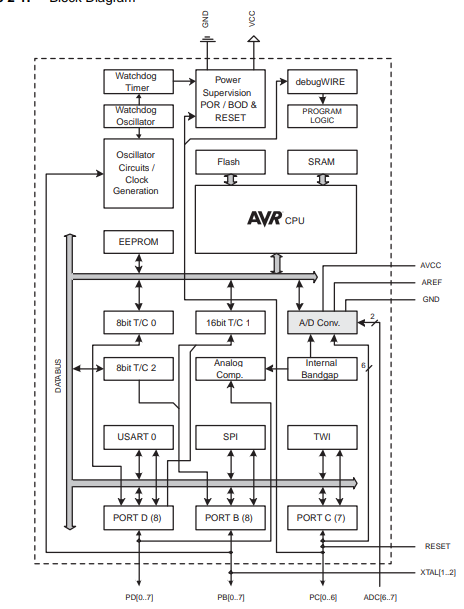
\includegraphics[width=.8\linewidth]{Imagenes/1.png}
% \caption{Pines del ATtiny4313. Tomado de \cite{web}.}
% \label{fig1}
%\end{figure}
%%%
\subsubsection*{Características generales}

\subsection*{Periféricos}
\subsection*{Componentes electrónicos complementarios}
\subsubsection*{Decodificador BCD y display de 7 segmentos}
    
\subsection*{Lista de componentes}

\begin{table}[H]
\caption{Lista de equipos}
\label{table_2}
\begin{center}
\begin{tabular}{r|cc}
\hline
\textbf{Componente}&\textbf{Cantidad}&\textbf{Precio}\\
 \hline
-&--  &-- \\ \hline 
 \textbf{Total}& &  \\
 \hline
\end{tabular}
\end{center}
\end{table}

\subsection*{Diseño del circuito}
\newpage
